% This LaTeX was auto-generated from MATLAB code.
% To make changes, update the MATLAB code and export to LaTeX again.

\documentclass{article}

\usepackage[utf8]{inputenc}
\usepackage[T1]{fontenc}
\usepackage{lmodern}
\usepackage{graphicx}
\usepackage{color}
\usepackage{hyperref}
\usepackage{amsmath}
\usepackage{amsfonts}
\usepackage{epstopdf}
\usepackage[table]{xcolor}
\usepackage{matlab}
\usepackage[paperheight=795pt,paperwidth=614pt,top=72pt,bottom=72pt,right=72pt,left=72pt,heightrounded]{geometry}

\sloppy
\epstopdfsetup{outdir=./}
\graphicspath{ {./Taller1_punto2_media/} }

\begin{document}

\matlabtitle{Punto 2}

\matlabheading{2.Diagonally scaled steepest descent method}

\begin{par}
\begin{flushleft}
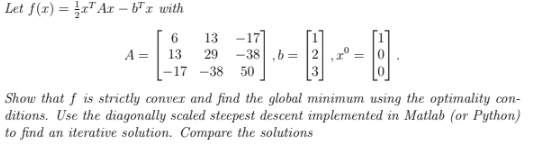
\includegraphics[width=\maxwidth{53.587556447566485em}]{image_0}
\end{flushleft}
\end{par}

\begin{matlabcode}
% Declaración de variables simbólicas
syms x1 x2 x3 real
x = [x1; x2; x3]

% Matriz A y vector b
A = [6, 13, -17;
     13, 29, -38;
     -17, -38, 50]
\end{matlabcode}
\begin{matlaboutput}
A = 3x3    
     6    13   -17
    13    29   -38
   -17   -38    50

\end{matlaboutput}
\begin{matlabcode}
b = [1; 2; 3]
\end{matlabcode}
\begin{matlaboutput}
b = 3x1    
     1
     2
     3

\end{matlaboutput}
\begin{matlabcode}

% Función f(x)
f1 = (1/2) * x.' * A * x - b.' * x
\end{matlabcode}


\matlabheadingthree{Demostrar que es convexa}

\begin{par}
\hfill \break
\end{par}

\begin{matlabcode}
% Gradiente (primera derivada)
grad_f = gradient(f1, x);
disp('Gradiente de f(x):');
\end{matlabcode}
\begin{matlaboutput}
Gradiente de f(x):
\end{matlaboutput}
\begin{matlabcode}
disp(grad_f);

% Hessiana (segunda derivada), es la misma matriz A
Hessian_f = hessian(f1, x);
disp('Hessiana de f(x):');
\end{matlabcode}
\begin{matlaboutput}
Hessiana de f(x):
\end{matlaboutput}
\begin{matlabcode}
disp(Hessian_f);

% 1. Verificación con valores propios
fprintf('1. Verificación de definida positiva usando valores propios:\n');
\end{matlabcode}
\begin{matlaboutput}
1. Verificación de definida positiva usando valores propios:
\end{matlaboutput}
\begin{matlabcode}
eigenvalues = eig(A);  % Calcula los valores propios de A
disp('Valores propios de A:');
\end{matlabcode}
\begin{matlaboutput}
Valores propios de A:
\end{matlaboutput}
\begin{matlabcode}
disp(eigenvalues);
\end{matlabcode}
\begin{matlaboutput}
    0.0588
    0.2007
   84.7405
\end{matlaboutput}
\begin{matlabcode}

if all(eigenvalues > 0)
    fprintf('La matriz A es definida positiva porque todos sus valores propios son positivos.\n\n');
else
    fprintf('La matriz A no es definida positiva porque no todos sus valores propios son positivos.\n\n');
end
\end{matlabcode}
\begin{matlaboutput}
La matriz A es definida positiva porque todos sus valores propios son positivos.
\end{matlaboutput}

\matlabheadingthree{Hallar el mínimo global con las Condiciones de optimalidad}

\begin{par}
\begin{flushleft}
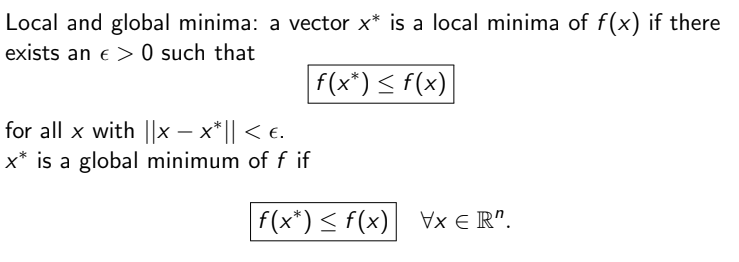
\includegraphics[width=\maxwidth{39.63873557451079em}]{image_1}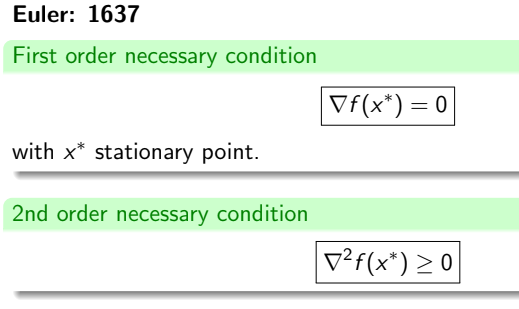
\includegraphics[width=\maxwidth{34.62117410938284em}]{image_2}
\end{flushleft}
\end{par}

\begin{matlabcode}
X = A \ b; % Este comando en Matlab resuelve las ecuaciones de forma Ax=B.
% Mostrar el resultado
disp('El mínimo global de la función se alcanza en:');
\end{matlabcode}
\begin{matlaboutput}
El mínimo global de la función se alcanza en:
\end{matlaboutput}
\begin{matlabcode}
disp(X);
\end{matlabcode}
\begin{matlaboutput}
   -5.0000
   39.0000
   28.0000
\end{matlaboutput}
\begin{matlabcode}

%Verificación
F=(1/2) * X.' * A * X - b.' * X
\end{matlabcode}
\begin{matlaboutput}
F = -78.5000
\end{matlaboutput}
\begin{matlabcode}
F2=gradient(F)
\end{matlabcode}
\begin{matlaboutput}
F2 = 0
\end{matlaboutput}

\matlabheadingthree{Método de descenso más pronunciado en escala diagonal}

\begin{par}
\begin{flushleft}
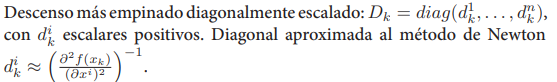
\includegraphics[width=\maxwidth{49.37280481685901em}]{image_3}
\end{flushleft}
\end{par}

\begin{matlabcode}
grad_x1 = @(x1,x2,x3) (6*x1 + 13*x2 - 17*x3 - 1)
\end{matlabcode}
\begin{matlaboutput}
grad_x1 = function_handle with value:
    @(x1,x2,x3)(6*x1+13*x2-17*x3-1)

\end{matlaboutput}
\begin{matlabcode}
grad_x2 = @(x1,x2,x3) (13*x1 + 29*x2 - 38*x3 - 2)
\end{matlabcode}
\begin{matlaboutput}
grad_x2 = function_handle with value:
    @(x1,x2,x3)(13*x1+29*x2-38*x3-2)

\end{matlaboutput}
\begin{matlabcode}
grad_x3 = @(x1,x2,x3) (50*x3 - 38*x2 - 17*x1 - 3)
\end{matlabcode}
\begin{matlaboutput}
grad_x3 = function_handle with value:
    @(x1,x2,x3)(50*x3-38*x2-17*x1-3)

\end{matlaboutput}
\begin{matlabcode}

f2=matlabFunction(f1)
\end{matlabcode}
\begin{matlaboutput}
f2 = function_handle with value:
    @(x1,x2,x3)-x1-x2.*2.0-x3.*3.0+x1.*(x1.*3.0+x2.*(1.3e+1./2.0)-x3.*(1.7e+1./2.0))-x3.*(x1.*(1.7e+1./2.0)+x2.*1.9e+1-x3.*2.5e+1)+x2.*(x1.*(1.3e+1./2.0)+x2.*(2.9e+1./2.0)-x3.*1.9e+1)

\end{matlaboutput}
\begin{matlabcode}
% Valores iniciales
pts2(1,1) = 1;  % Valor inicial para x1
pts2(1,2) = 0;  % Valor inicial para x2
pts2(1,3) = 0;  % Valor inicial para x3
step = 0.6           % Paso (alpha)
\end{matlabcode}
\begin{matlaboutput}
step = 0.6000
\end{matlaboutput}
\begin{matlabcode}
max_iters = 30000       % Número máximo de iteraciones
\end{matlabcode}
\begin{matlaboutput}
max_iters = 30000
\end{matlaboutput}
\begin{matlabcode}
tolerancia = 1e-3      % Tolerancia para la convergencia
\end{matlabcode}
\begin{matlaboutput}
tolerancia = 1.0000e-03
\end{matlaboutput}


\begin{matlabcode}
% Algoritmo de descenso más pronunciado con escala diagonal
i = 1;
for i = 1:max_iters
    % Gradiente en el punto actual
    gradix1 = grad_x1(pts2(i,1), pts2(i,2),pts2(i,3));  % Evaluar derivada parcial en x1
    gradix2 = grad_x2(pts2(i,1), pts2(i,2),pts2(i,3));  % Evaluar derivada parcial en x2
    gradix3 = grad_x3(pts2(i,1), pts2(i,2),pts2(i,3));  % Evaluar derivada parcial en x3

    % Escala diagonal D (tomamos la diagonal de A, en este caso como ejemplo, la diagonal de A)
    D = diag([1/A(1,1), 1/A(2,2), 1/A(3,3)]);  % Usamos las primeras dos entradas de la matriz A

    % Calculamos el siguiente paso de x1 y x2 (descenso con escala diagonal)
    pts2(i+1,1) = pts2(i,1) - step * D(1,1) * gradix1; % Actualización de x1
    pts2(i+1,2) = pts2(i,2) - step * D(2,2) * gradix2; % Actualización de x2
    pts2(i+1,3) = pts2(i,3) - step * D(3,3) * gradix3; % Actualización de x3
    % Visualización de la evolución de las variables
    plot( f2(pts2(i+1,1), pts2(i+1,2), pts2(i+1,3)), pts2(i+1,1), '.-', 'LineWidth', 1, 'Color', '#0072BD', 'DisplayName', 'x1');
    hold on;
    plot( f2(pts2(i+1,1), pts2(i+1,2), pts2(i+1,3)), pts2(i+1,2), '.-', 'LineWidth', 1, 'Color', '#D95319', 'DisplayName', 'x2');
    hold on;
    plot( f2(pts2(i+1,1), pts2(i+1,2), pts2(i+1,3)), pts2(i+1,3), '.-', 'LineWidth', 1, 'Color', '#EDB120', 'DisplayName', 'x3');
    hold on;
    % Verificar condición de convergencia (gradiente suficientemente pequeño)
    if (abs(gradix1) < tolerancia) && (abs(gradix2) < tolerancia) && (abs(gradix3) < tolerancia)
        break;  % Converge si el gradiente es suficientemente pequeño  
    end
end
\end{matlabcode}
\begin{center}
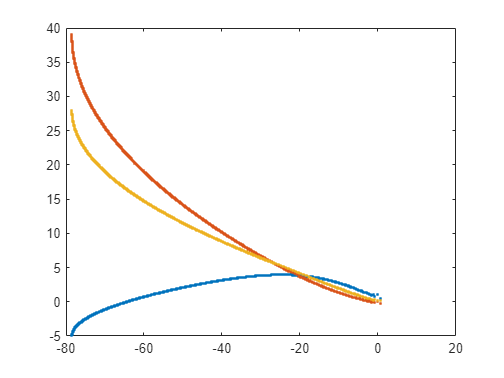
\includegraphics[width=\maxwidth{50.57701956848972em}]{figure_0.png}
\end{center}
\begin{matlabcode}

% Mostrar el resultado final
fprintf("Se alcanzó el objetivo en %d iteraciones\n", i)
\end{matlabcode}
\begin{matlaboutput}
Se alcanzó el objetivo en 7236 iteraciones
\end{matlaboutput}
\begin{matlabcode}
fprintf("El punto final es (x1=%1.2f, x2=%1.2f, z=%1.2f)\n", pts2(end,1), pts2(end,2), pts2(end,3))
\end{matlabcode}
\begin{matlaboutput}
El punto final es (x1=-5.00, x2=38.98, z=27.99)
\end{matlaboutput}

\end{document}
